\documentclass{exam}

\usepackage[top=0.9in, bottom=1in, left=1.5in, right=1.5in]{geometry}
\usepackage[utf8]{inputenc}
\usepackage[icelandic]{babel}
\usepackage[T1]{fontenc}
\usepackage[sc]{mathpazo}

\usepackage[parfill]{parskip}
\usepackage{booktabs,tabularx}
\usepackage{multirow}
\usepackage{enumerate}
\usepackage{graphicx}
\usepackage{amsmath, amsfonts, amssymb, amsthm}
\usepackage{tikz}
\makeatletter % Fix due to (recent versions of?) minted containing their own framed definition
\expandafter\providecommand\expandafter*\csname ver@framed.sty\endcsname
{2003/07/21 v0.8a Simulated by exam}
\makeatother
\usepackage{minted} %Minted and configuration

\usepackage[pdftex,bookmarks=true,colorlinks=true,pdfauthor={Eirikur Ernir Thorsteinsson},linkcolor=blue,urlcolor=blue]{hyperref}

\setcounter{secnumdepth}{-1} 
\hyphenpenalty=5000


% Picture locations
\graphicspath{{./Pics/}}

\usemintedstyle{default}
\renewcommand{\theFancyVerbLine}{\sffamily \arabic{FancyVerbLine}}

\newcommand{\Mod}[1]{\ \text{mod}\ #1}

\runningfooter{\hspace{-2cm}
\includegraphics[width=0.5\textwidth]{Pics/hi-von-logo}}{}{}

\renewcommand{\solutiontitle}{\noindent\textbf{Mögulegt svar:}}

\author{}
\date{}

\footer{}{}{}


\title{Stærðfræðimynstur í tölvunarfræði \\ Skilaverkefni 11}
\author{}

\printanswers

\begin{document}
\maketitle
\thispagestyle{empty} 

Skila skal þessu verkefni á vefnum \href{https://gradescope.com/}{Gradescope}. Aðgangskóði fyrir námskeiðið er \textbf{926WD9}.


\section{Spurningar}

\begin{questions}

\section{Kafli 10.7}

\question Eru eftirfarandi net lagnet? Sé svo, teiknið tilsvarandi sléttunet. Sé svo ekki, gefið ástæðu.

\begin{center}
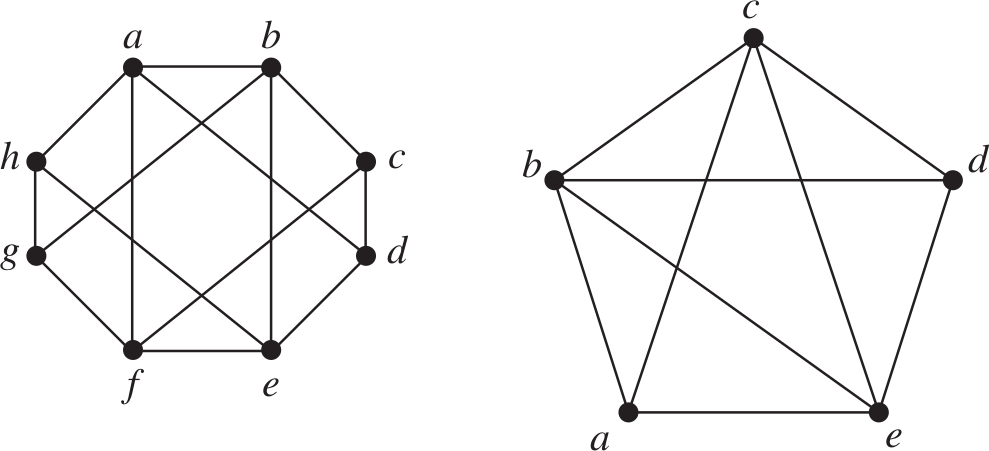
\includegraphics[width=0.5\textwidth]{graph-maybe-planar}
\end{center}

\paragraph{Í bók:} Byggt á fyrstu æfingum í kafla 10.7.

\section{Kafli 10.8}

\question Fjarlægðir á milli sex útvarpssendistöðva í kílómetrum eru gefnar á eftirfarandi töflu.

\begin{center}

\begin{tabular}{ccccccc}
\toprule
&1&2&3&4&5&6\\
\midrule
1&-&85&175&200&50&100\\
2&85&-&125&175&100&160\\
3&175&125&-&100&200&250\\
4&200&175&100&-&210&220\\
5&50&100&200&210&-&100\\
6&100&160&250&220&100&-\\
\bottomrule
\end{tabular}

\end{center}
Hversu margar mismunandi útvarprásir þurfa þessar stöðvar, ef tvær stöðvar geta ekki notað sömu rásina séu þær innan 150 kílómetra hver frá annarri?

Leysið verkefnið með því að setja fram net og ákvarða fyrir það litunartölu.

\paragraph{Í bók:} Exercise 10.8.18

\section{Kaflar 10 og 11}

\question Öll tré með a.m.k. tvo hnúta eru tvíhlutanet. Rökstyðjið.

\paragraph{Í bók:} Þetta dæmi er ekki í bókinni.

\section{Kafli 10.1}

\question Gefið er eftirfarandi rótartré:

\begin{center}
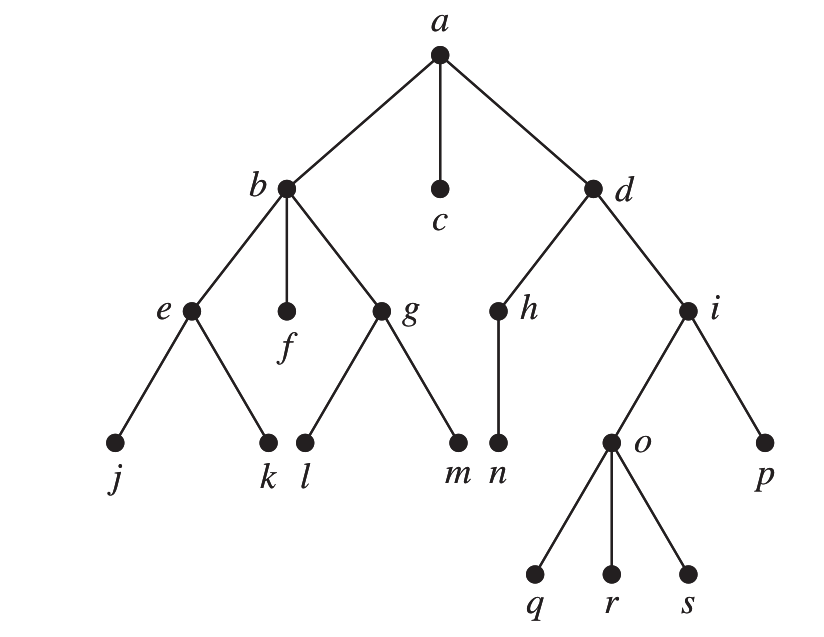
\includegraphics[width=0.6\textwidth]{tree-exercise}
\end{center}

\begin{enumerate}[a)]
 \item Hvaða hnútur er rótin?
 \item Hvaða hnútar eru innri hnútar?
 \item Hvaða hnútar eru lauf?
 \item Hvaða hnútar eru börn $j$?
 \item Hvaða hnútur er foreldri $h$?
 \item Hvaða hnútar eru systkini $o$?
 \item Hvaða hnútar eru áar $m$?
 \item Hvaða hnútar eru afkomendur $b$?
\end{enumerate}
Einungis upptalning á viðkomandi hnútum er nauðsynleg í hverjum lið.

\paragraph{Í bók:} Exercise 10.1.4

\question Keðjubréf nokkurt byrjar þegar manneskja sendir bréfið á fimm aðrar manneskjur. Allir sem fá bréfið senda það annaðhvort til fimm annarra sem ekki hafa fengið bréfið áður eða senda það ekki áfram á neinn.

Gefum okkur að 10000 manneskjur sendi bréfið áður en það fjaraði út og að enginn fái bréfið tvisvar. Hversu margir fengu bréfið og hve margir sendu það ekki áfram? Útskýrið með hugtökum sem tengjast trjám.

\paragraph{Í bók:} Exercise 10.1.22

\section{Kafli 10.2}

\question Getur leikmaður $x$ alltaf unnið í eftirfarandi stöðu í myllu?

\begin{center}
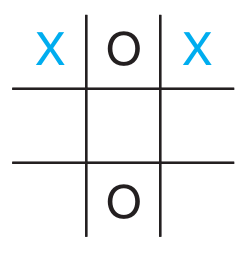
\includegraphics[width=0.25\textwidth]{tic-tac-toe-exercise}
\end{center}

Leysið verkefnið með því að teikna upp og greina leikjatré.

\paragraph{Í bók:} Exercise 10.2.38

\end{questions}


\end{document}